\documentclass[a4paper]{article}

%% Language and font encodings
\usepackage[english]{babel}
\usepackage[utf8x]{inputenc}
\usepackage[T1]{fontenc}

%% Sets page size and margins
\usepackage[a4paper,top=3cm,bottom=2cm,left=3cm,right=3cm,marginparwidth=1.75cm]{geometry}

%% Useful packages
\usepackage{amsmath}
\usepackage{graphicx}
\usepackage{subcaption}
\usepackage[colorinlistoftodos]{todonotes}
\usepackage[colorlinks=true, allcolors=blue]{hyperref}

\title{Investigating Blip Glitches Using GravitySpy and Q-Transforms to Find Sub-Classes}
\author{Melissa Kohl}
\date{\today}

\begin{document}
\maketitle
\graphicspath{ {images/} }

\begin{abstract}

In the Advanced LIGO observation runs, detection of gravitational waves is directly dependent on the sensitivity of the detectors. The strain data contain noise called "glitches" that mimic and obscure real gravitational waves. The machine learning software package used to classify these glitches and identify their sources, GravitySpy, is successful when the spectrogram of the glitch has a very distinct and unique shape. However, the spectrogram of one of the most common types of glitches, called a "blip," has an underwhelming shape with no distinct characteristics, making it difficult for GravitySpy to identify a source (or possibly multiple sources). This suggests looking at blip glitches in a format other than a spectrogram, such as a Q-transform, to determine if there are sub-classifications of blips that might have identifiable sources. Fortunately, the Q-transforms of a variety of blip glitches, nearly indistinguishable in a spectrogram, reveal distinct possible subclasses.

\end{abstract}

\section{Introduction to Glitch Classification} \label{introduction}

The glitches in the strain data from the science and observation runs of the Advanced LIGO detectors decrease the sensitivity of the detectors and obscure gravitational waves \cite{Zevin:2016}. Although some glitches can be identified and eliminated from the strain data during later analysis, astronomical events that give off additional radiation, such as neutron star mergers, need to be recognized immediately so that astronomers can observe the event. Additionally, the shapes of some glitches, such as "blip" glitches, mimic that of a gravitational wave from a binary black hole merger so well that one of the only ways to distinguish a blip from a gravitational wave is by comparing the data between detectors. As a result, it is imperative to find the sources of the glitches and eliminate them before future observing runs, directly increasing the sensitivity of the detectors while observing \cite{Mukherjee:2010}. 

The current method for classifying glitches and identifying their sources is a machine learning software package called GravitySpy \cite{Zevin:2016}. Unlike previous machine learning techniques used on LIGO data that only looked at the waveforms of the glitches \cite{Mukherjee:2010}, GravitySpy's neural network takes in spectrograms from four different time frames to create a multi-layer network that utilizes image classification techniques \cite{Bahaadini:2017}. Since different types of glitches have different durations, the multiple views not only provide complementary data across time frames, but also allow for identification of a broader group of glitches of different durations \cite{Bahaadini:2017}. GravitySpy is therefore great at classifying glitches into known classifications \cite{Zevin:2016}, but the classifications themselves may be too broad. The output function in GravitySpy's neural network is \textit{softmax} \cite{Bahaadini:2017}, which essentially just classifies the input glitch into the classification with the highest correlation, regardless of how high that correlation is. The combination of the multiple-view input and the \textit{softmax} output function allow for glitches caused by different sources to be classified into the same group if the shapes of the glitches are similar. In section \ref{investigation}, I introduce an example of two different spectrogram shapes (which most likely have different sources) that are grouped into the same classification. 

Once glitches are classified, GravitySpy is also used to find similar glitches in the hundreds of thousands of auxiliary channels keeping track of the instruments and environments of each detector in an attempt to locate the source of each glitch classification \cite{Zevin:2016}. Currently, this method is insufficient for finding the source of common glitch classifications such as blips.

\section{Initial Approach and Goals} \label{goal}

The most frequently-occurring glitches, including blip glitches, are likely conglomerates of glitches from different sources that happen to create the same general shape in a spectrogram. Unfortunately, the shape of a blip glitch in a spectrogram is uninspiring, with no weird spikes or unique shapes to provide a hint towards its source, and little to even distinguish one from another. To sub-classify these blip glitches, we first need a different analysis technique that might reveal hidden characteristics. 

One common way to visualize a glitch or other transient noise waveform in the strain data is a Q-transform, which is a time-to-frequency domain transform related to the Fourier transform. The quality factor Q is related to the number of cycles processed at a central frequency, and in comparison with a Fourier transform, the Q-transform has a better frequency resolution over a logarithmic frequency scale. Since the glitches and gravitational waves in the Advanced LIGO strain data span auditory frequencies, which are on a logarithmic scale, the Q-transform is a more desirable time-to-frequency domain transform than the Fourier transform. 

If blip glitches do have distinguishable subclasses, we can create a new input set with these subclassifications to put into GravitySpy's neural network. Without sub-classification, GravitySpy cannot identify the sources of blip glitches, but with a new input set, the possibility of finding a source and reducing some of the noise caused by blip glitches is largely increased. 

\section{Investigation of Blip Glitches} \label{investigation}

To gain a better understanding of blip glitches and their characteristics, I started by performing Q-transforms on known glitches from the first observing run at the Livingston detector. I wrote a Python script, adapted from the GWpy Q-transform documentation, to plot the Q-transform of about 30 random glitches, all cropped from the surrounding 30 seconds of strain data to a final image with a time domain of 0.30 seconds. While manually looking through the images, I found four distinct types of blip glitches, as seen in figure \ref{fig:q_transforms}. I called the four types normal, spread, dot, and stick for their appearances in the Q-transform, but there was a lot more investigation needed before making the assumption that these were indeed sub-classes.

\begin{figure}[h!]
	\centering
	\begin{subfigure}{.49\textwidth}
		\centering
		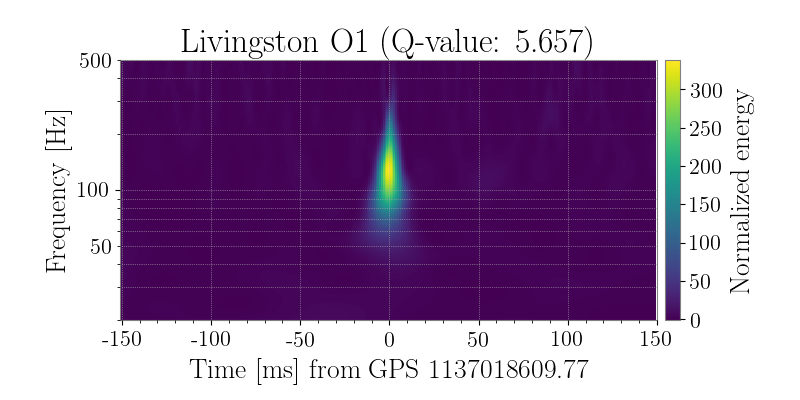
\includegraphics[width=1\linewidth]{normal_blip}
		\caption{Normal blip Q-transform}
		\label{fig:normal}
	\end{subfigure}
	\begin{subfigure}{.49\textwidth}
		\centering
		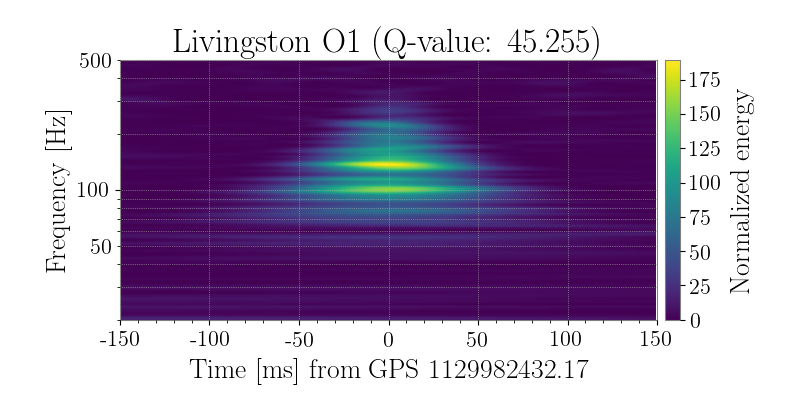
\includegraphics[width=1\linewidth]{spread_blip}
		\caption{Spread blip Q-transform}
		\label{fig:spread}
	\end{subfigure}
	\begin{subfigure}{.49\textwidth}
		\centering
		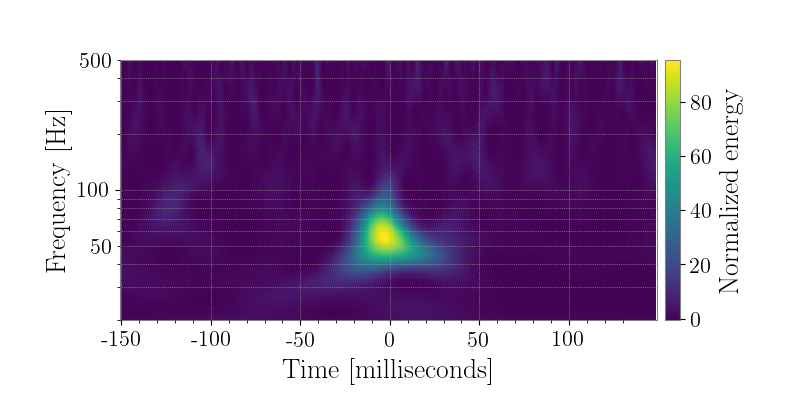
\includegraphics[width=1\linewidth]{dot_blip}
		\caption{Dot blip Q-transform}
		\label{fig:dot}
	\end{subfigure}
	\begin{subfigure}{.49\textwidth}
		\centering
		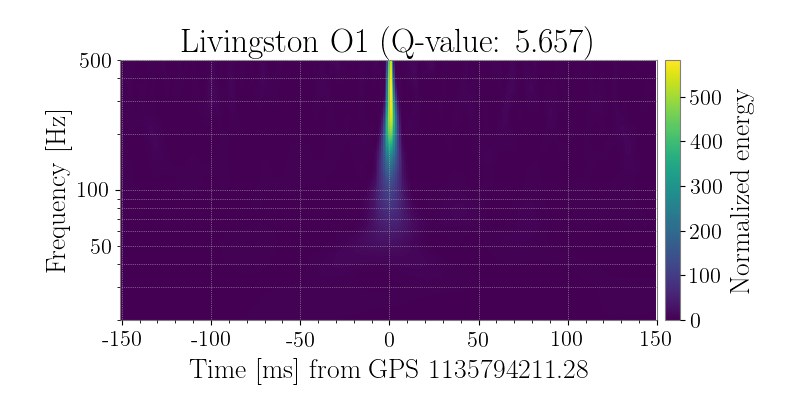
\includegraphics[width=1\linewidth]{stick_blip}
		\caption{Stick blip Q-transform}
		\label{fig:stick}
	\end{subfigure}
	\caption{Four different types of blip glitches in Q-transforms, all with the same time duration of 0.30 seconds, cropped from 30 seconds of transformed strain data.}
	\label{fig:q_transforms}
\end{figure}

After discovering these differing forms in the Q-transforms and plotting about 100 more Q-transforms, I looked at the existing spectrograms from LigoDV-Web of a specific glitch from each of the four possible subclassifications to determine the legitimacy of my assumptions, the results of which are in figure \ref{fig:comparison} below. 

\begin{figure}[h!]
	\centering
	\begin{subfigure}[t]{.7\textwidth}
		\centering
		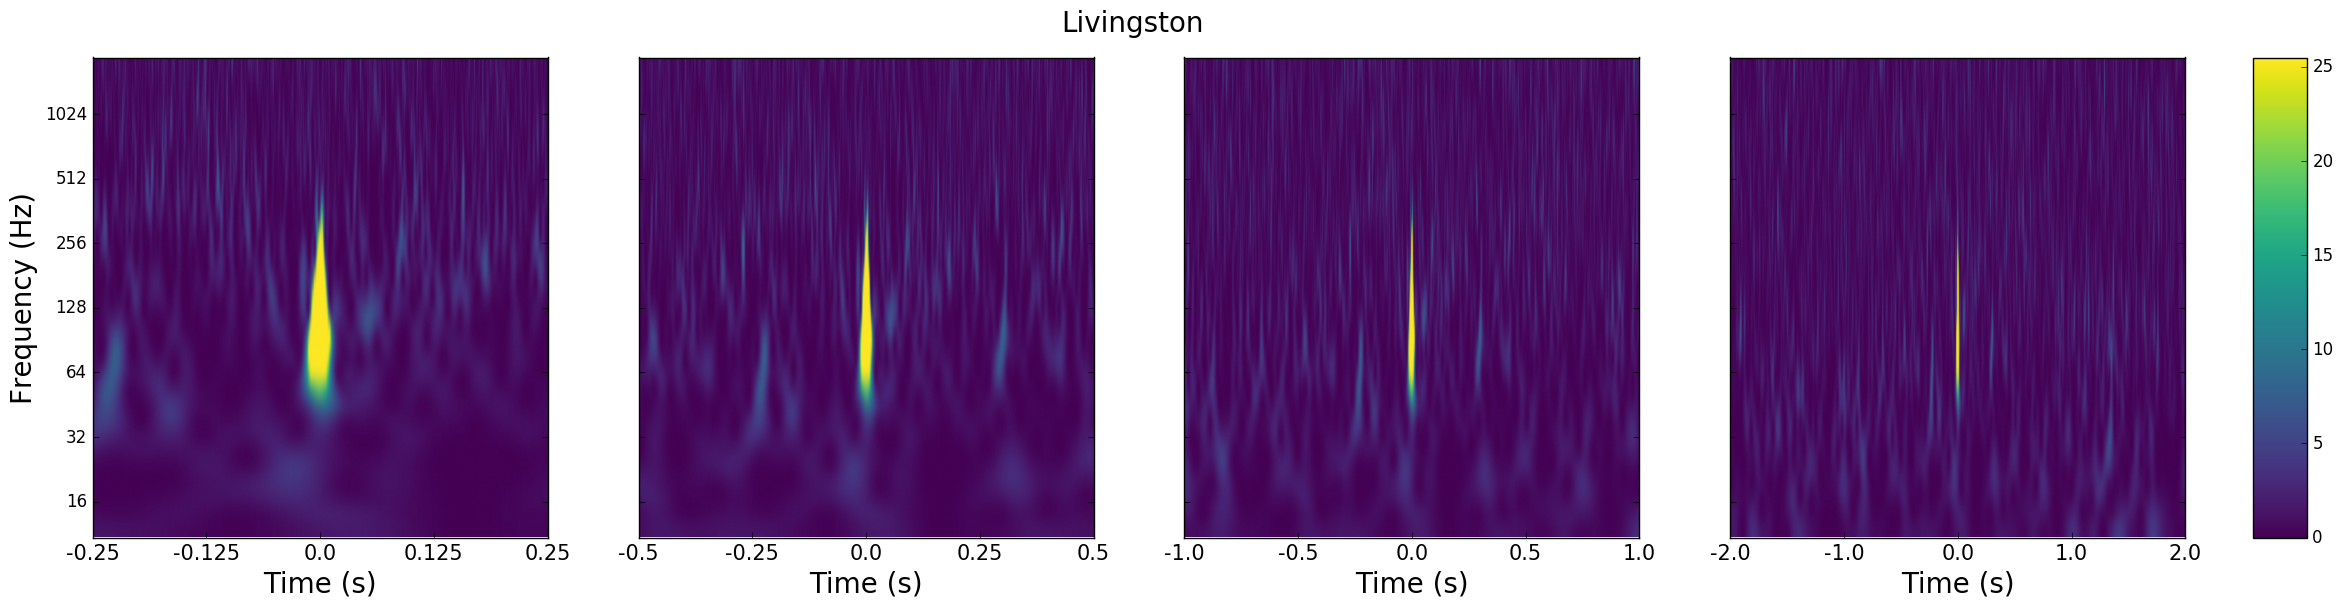
\includegraphics[width=.9\linewidth]{normal_blip_spect}
		\caption{Normal blip spectrograms}
		\label{fig:normal_s}
	\end{subfigure}
	\begin{subfigure}[t]{.29\textwidth}
		\centering
		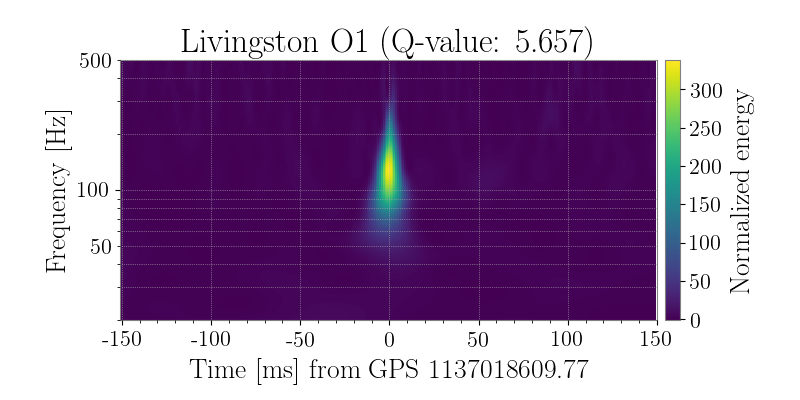
\includegraphics[width=1.1\linewidth]{normal_blip}
		\caption{Normal blip Q-transform}
		\label{fig:normal_q}
	\end{subfigure}
	\begin{subfigure}[t]{.7\textwidth}
		\centering
		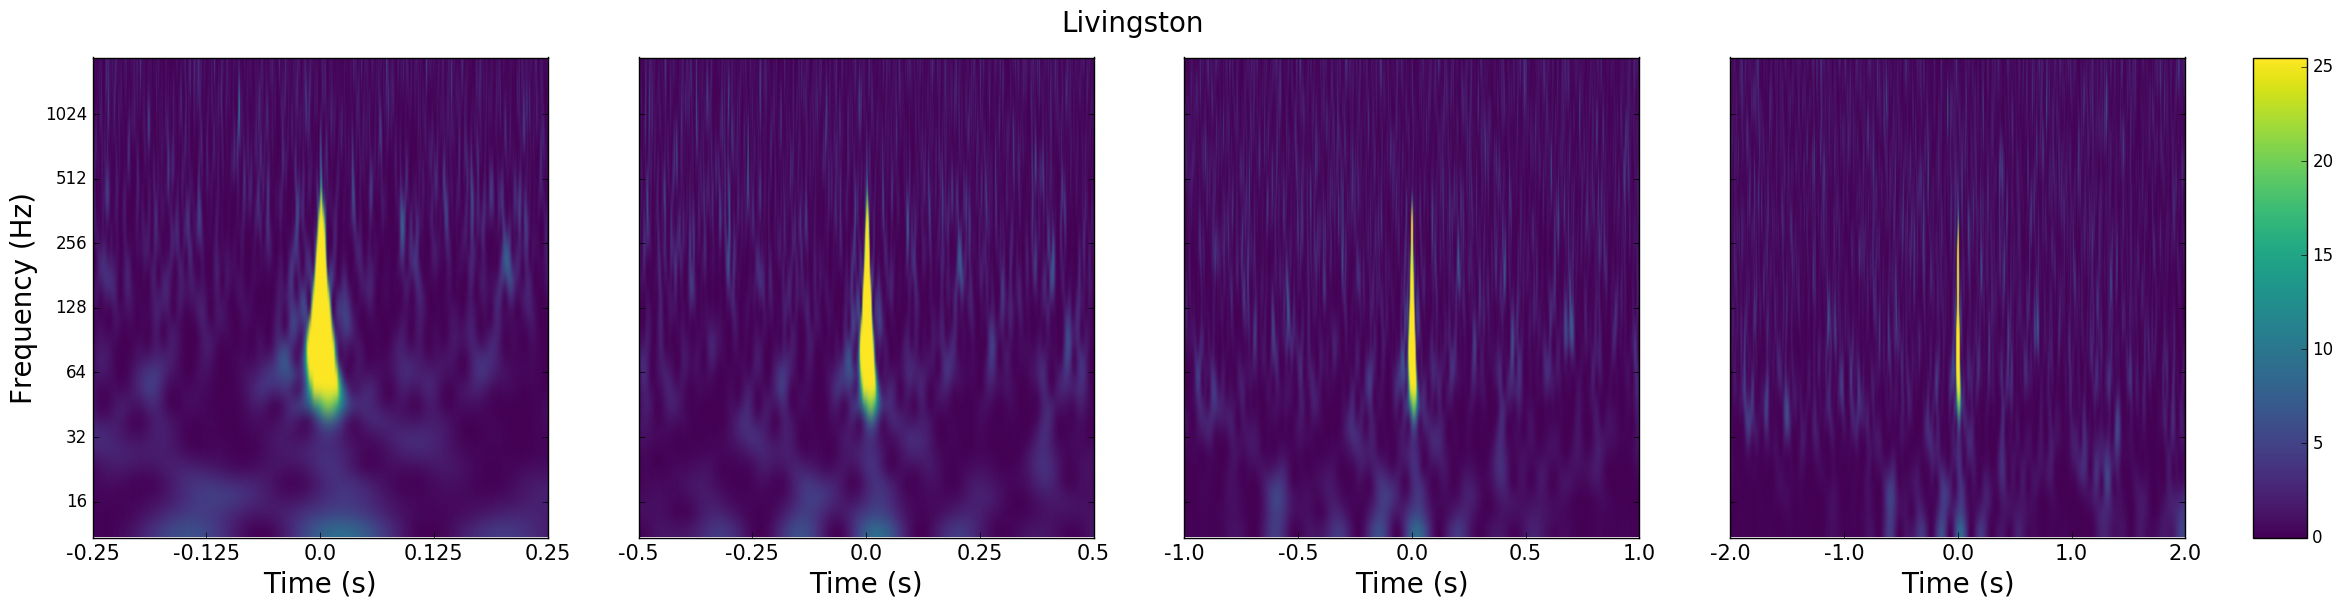
\includegraphics[width=.9\linewidth]{spread_blip_spect}
		\caption{Spread blip spectrograms}
		\label{fig:spread_s}
	\end{subfigure}
	\begin{subfigure}[t]{.29\textwidth}
		\centering
		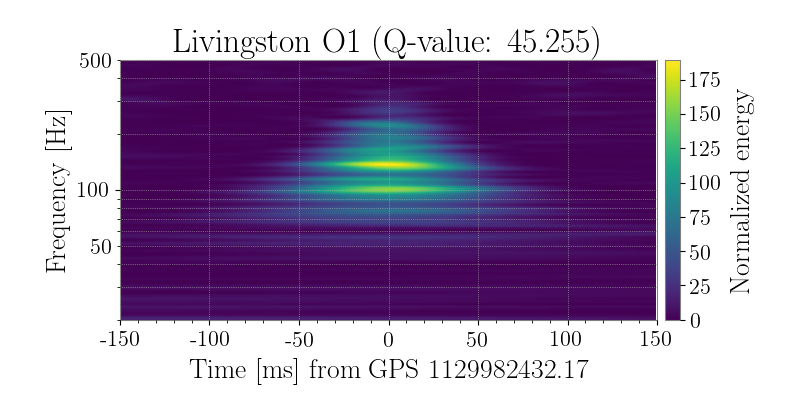
\includegraphics[width=1.1\linewidth]{spread_blip}
		\caption{Spread blip Q-transform}
		\label{fig:spread_q}
	\end{subfigure}
	\begin{subfigure}[t]{.7\textwidth}
		\centering
		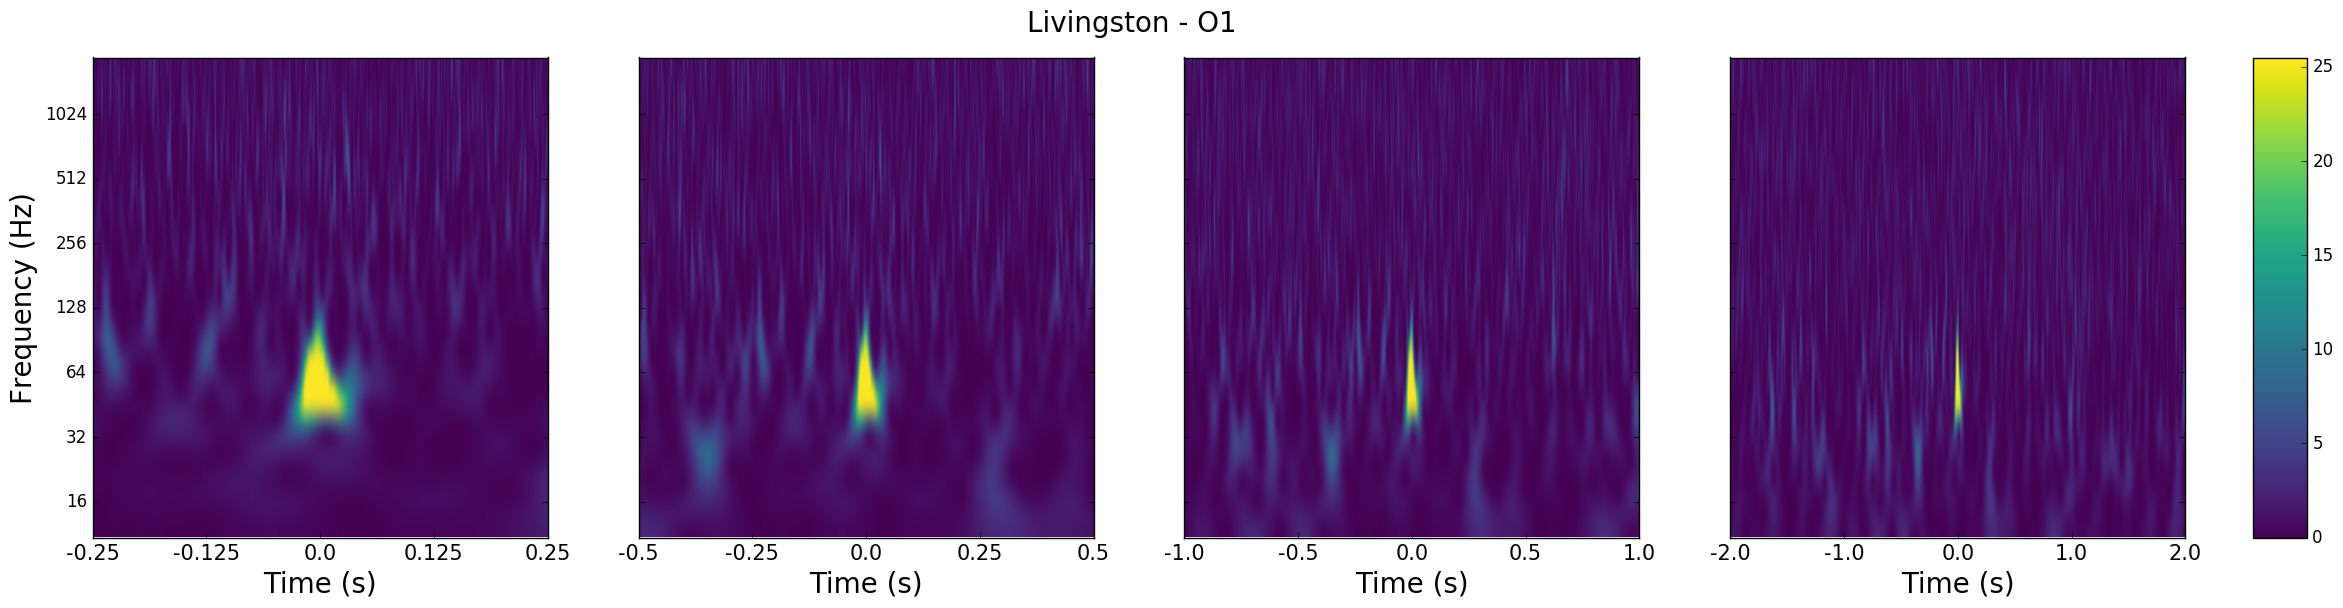
\includegraphics[width=.9\linewidth]{dot_blip_spect}
		\caption{Dot blip spectrograms}
		\label{fig:dot_s}
	\end{subfigure}
	\begin{subfigure}[t]{.29\textwidth}
		\centering
		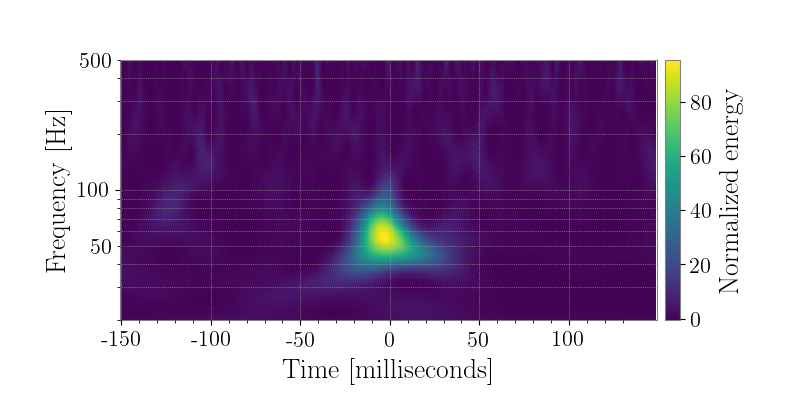
\includegraphics[width=1.1\linewidth]{dot_blip}
		\caption{Dot blip Q-transform}
		\label{fig:dot_q}
	\end{subfigure}
	\begin{subfigure}[t]{.7\textwidth}
		\centering
		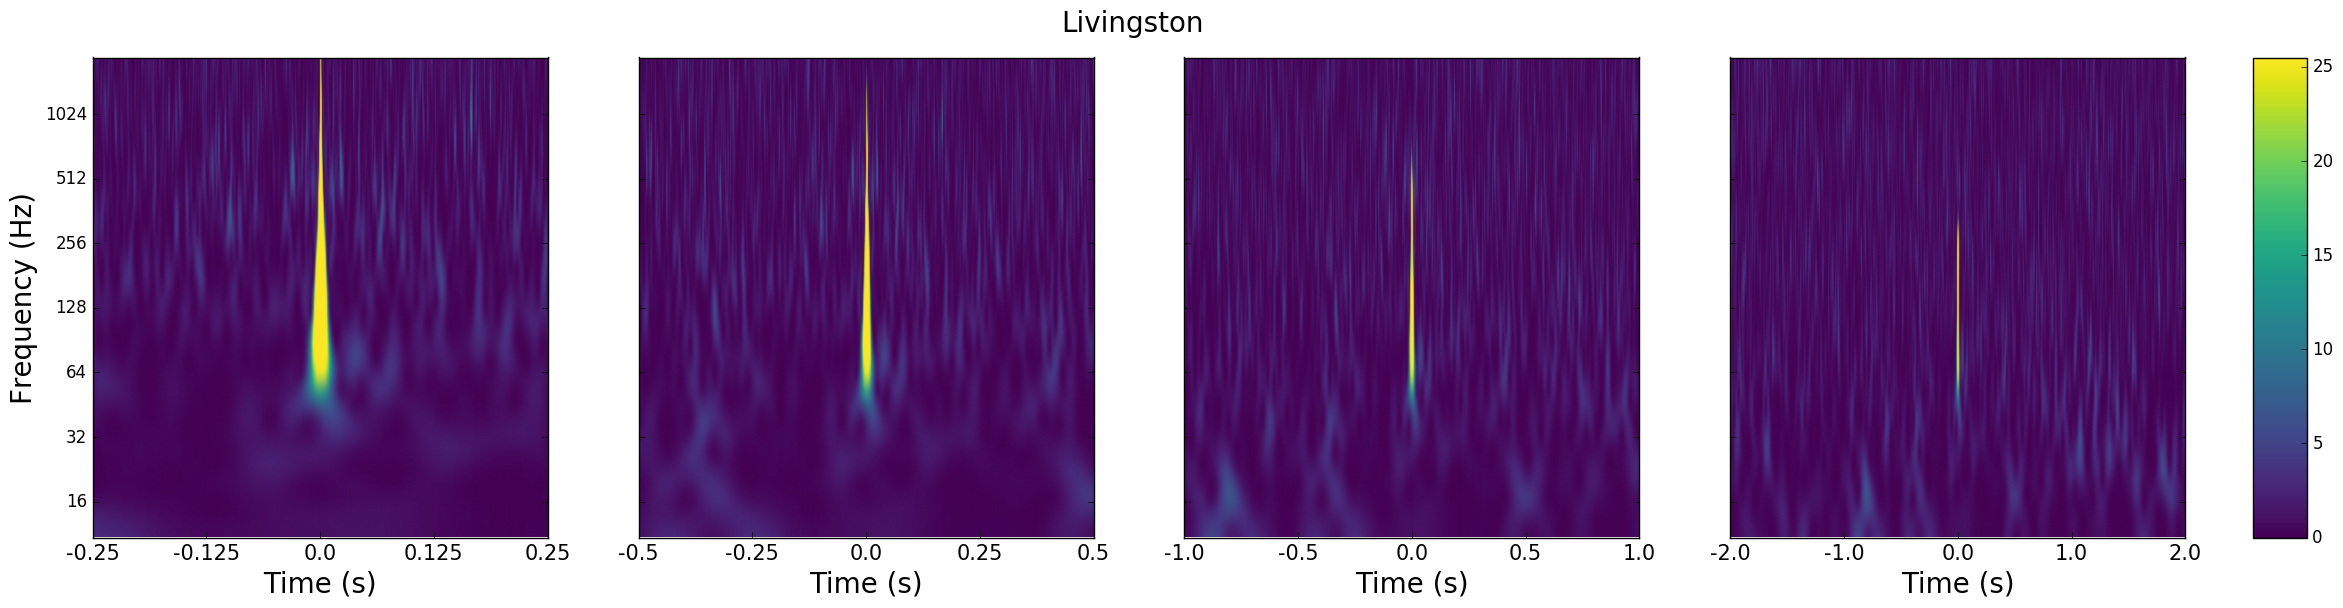
\includegraphics[width=.9\linewidth]{stick_blip_spect}
		\caption{Stick blip spectrograms}
		\label{fig:stick_s}
	\end{subfigure}
	\begin{subfigure}[t]{.29\textwidth}
		\centering
		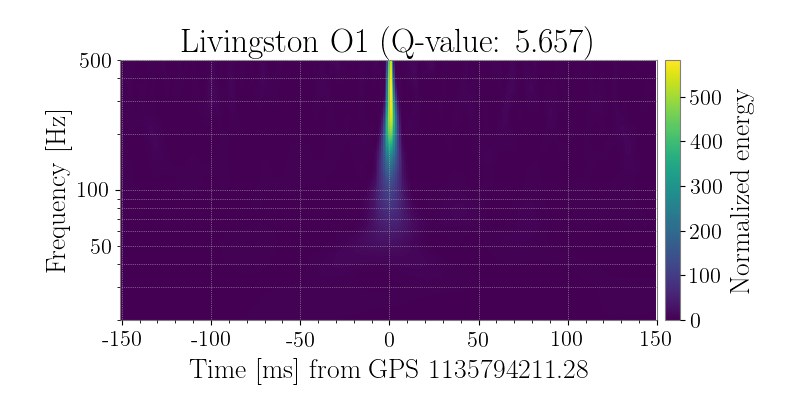
\includegraphics[width=1.1\linewidth]{stick_blip}
		\caption{Stick blip Q-transform}
		\label{fig:stick_q}
	\end{subfigure}
	\caption{A comparison between spectrograms of four different blip glitches on the left and the corresponding Q-transform of the same blip glitches on the right. The spectrogram images come from LigoDV-Web, with time durations from left to right of 0.5 seconds, 1.0 seconds, 2.0 seconds, and 4.0 seconds. The Q-transform images were created from my Python script, cropped from 30 seconds of transformed data down to 0.30 seconds. The top row is a normal blip, the second row is a spread blip, the third a dot blip, and a stick blip on the bottom. Although the spectrograms of the different blips are distinguishable from one another, the Q-transforms reveal that these blip glitches are fundamentally different.}
	\label{fig:comparison}
\end{figure}

The most striking difference between the spectrograms and the Q-transforms is from the spread blip. The spectrograms from the normal blip and the spread blip, figures \ref{fig:normal_s} and \ref{fig:spread_s}, appear to be almost exactly the same, but while the normal blip's Q-transform (figure \ref{fig:normal_q}) has the same shape as its spectrogram, hence the name "normal," the spread blip's Q-transform (figure \ref{fig:spread_s}) "spreads" outward with distinct horizontal lines. The spread blip therefore has a good chance of being a true sub-classification of blip glitches. Additionally, the horizontal lines (which are essentially frequency bins) suggest that the duration of a spread blip is longer than the rest of the blips and therefore needs more data than 30 seconds for a clear Q-transform. 

The dot blip also has a chance of being a legitimate sub-classification, as its Q-transform (figure \ref{fig:dot_q}) has a distinct round shape at a relatively low frequency compared to the other blips. Unlike the spread blip, however, the spectrogram of the dot blip (figure \ref{fig:dot_s}) is easily distinguishable from the others, with a much smaller frequency range and an almost triangle-like shape. This is an example of a possible distinguishable classification of glitch that GravitySpy groups in with blips, as mentioned in the section \ref{introduction}. So, since a dot blip can be identified on a spectrogram, it is possible that it could be classified apart from other blip glitches by GravitySpy, but it is worth investigating possible attributes of dot blips, such as lower frequency and longer duration compared to other blips.

The stick blip also seems to be different than a normal blip. Its spectrogram (figure \ref{fig:stick_s}) is only slightly skinnier than that of a normal blip, with a slightly longer tail. However, the Q-transform (figure \ref{fig:stick_q}) reveals that a stick blip is at a significantly higher frequency than a normal blip. Even if the stick blip is the same shape as a normal blip, the higher frequency sets it apart, especially compared to dot blips.

\section{Determining Distinguishable Characteristics of Possible Sub-Classifications of Blip Glitches}

The first step I took in finding specific attributes to subclassify the blip glitches was sorting glitches by frequency, inspired by the apparent difference between dot blips and stick blips. First looking at blips with an SNR below 12, I modified my Python script to separate the Q-transforms into three peak-frequency bins: lower than 100 Hz, 100-200 Hz, and higher than 200 Hz. 

At low peak frequency, there were no stick blips and a few spreads, but mostly dots and normals. At mid peak frequency, there was a mix of all of the types but still no sticks. At high frequency, there were sticks and a few spreads. So, my assumption that stick blips occur at higher frequency than the rest still holds, but the dot blips couldn't be separated from normal blips based just on frequency. Additionally, the spread blips remain elusive, with a handful in each frequency range.

In an attempt to isolate the spread blips, I looked at blip glitches with different durations due to the apparent long duration of the spread blips compared to the others. Unfortunately, there were spread blips with both high duration and low duration. I then tried the combination of a high duration and low SNR, but again there was no distinction for the spread glitches. 

\section{Moving Forward}

Now that there are specific types of blip glitches to investigate, there are many avenues for further investigation into these four possible subclasses of blip glitches. Due to a limited knowledge of GravitySpy and GWpy, I have so far been limited to looking at blip glitches in O1, but I now know how to look at blip glitches in O2 and I can now investigate whether the same four types of blips exist in both observing runs. I have also been looking at only L1 data, so another next step is to look at the Hanford strain data for O1 and O2. 

Since the Q-transform images of the four different types of blips appear to have different peak frequencies, another possibility is to create a histogram of all the blip glitches and their peak frequencies to see if there are any groupings. I could also do the same thing with duration to see whether spread glitches actually do have a dependency on duration.

The other way to investigate the relationship between the spread blips and duration is to modify the initial duration of the Q-transform to possibly refine the image of the spread blips, assuming that they do have a longer duration compared to the other types of blips.

Once I have more information about these four possible blip subclassifications, I can begin working on creating a new input set for GravitySpy to attempt actually subclassifying blip glitches.


\bibliography{references}
\bibliographystyle{ieeetr}

\end{document}












